% Architecture diagram for the paper - compile standalone with pdflatex
\documentclass[tikz,border=10pt]{standalone}
\usepackage{tikz}
\usetikzlibrary{shapes.geometric,arrows.meta,positioning,fit,backgrounds}

\begin{document}
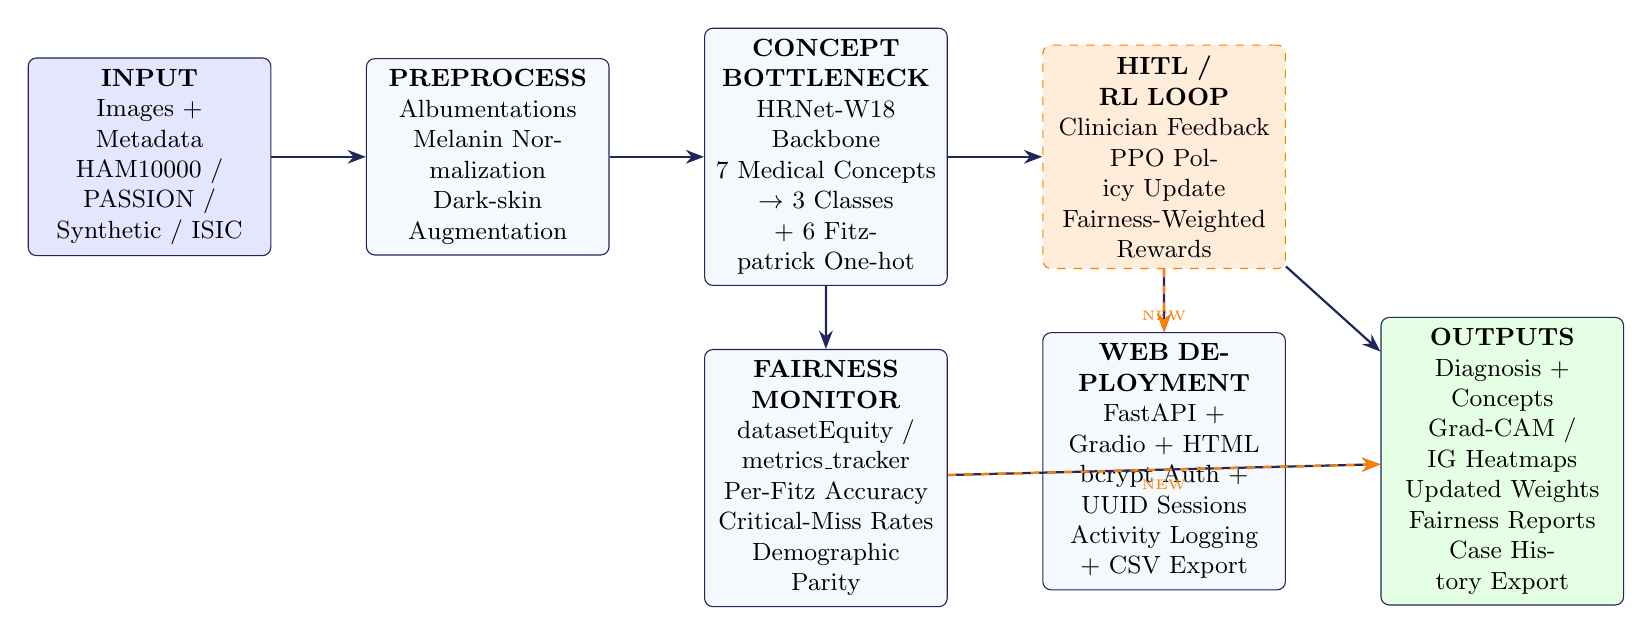
\begin{tikzpicture}[
    scale=0.85,
    node distance=8mm and 12mm,
    every node/.style={font=\small,align=center},
    box/.style={draw=darkblue,fill=boxbg,rounded corners=3pt,inner sep=4pt,minimum height=14mm,text width=2.8cm},
    arrow/.style={-Stealth,thick,darkblue},
    highlight/.style={fill=orange!15,draw=orange,dashed}
]

% Colors
\definecolor{darkblue}{RGB}{30,40,90}
\definecolor{boxbg}{RGB}{245,248,252}

% Row 1: Input -> Preprocess -> CBM -> HITL/RL
\node[box,fill=blue!10] (in) {\textbf{INPUT}\\\small Images + Metadata\\\small HAM10000 / PASSION / Synthetic / ISIC};
\node[box,right=of in] (prep) {\textbf{PREPROCESS}\\\small Albumentations\\\small Melanin Normalization\\\small Dark-skin Augmentation};
\node[box,right=of prep] (cbm) {\textbf{CONCEPT BOTTLENECK}\\\small HRNet-W18 Backbone\\\small 7 Medical Concepts $\to$ 3 Classes\\\small + 6 Fitzpatrick One-hot};
\node[box,right=of cbm,highlight] (hitl) {\textbf{HITL / RL LOOP}\\\small Clinician Feedback\\\small PPO Policy Update\\\small Fairness-Weighted Rewards};

% Row 2: Fairness Monitor -> Web Deploy -> Outputs
\node[box,below=of cbm] (fair) {\textbf{FAIRNESS MONITOR}\\\small datasetEquity / metrics\_tracker\\\small Per-Fitz Accuracy\\\small Critical-Miss Rates\\\small Demographic Parity};
\node[box,below=of hitl] (web) {\textbf{WEB DEPLOYMENT}\\\small FastAPI + Gradio + HTML\\\small bcrypt Auth + UUID Sessions\\\small Activity Logging + CSV Export};
\node[box,right=of web,fill=green!10] (out) {\textbf{OUTPUTS}\\\small Diagnosis + Concepts\\\small Grad-CAM / IG Heatmaps\\\small Updated Weights\\\small Fairness Reports\\\small Case History Export};

% Arrows
\draw[arrow] (in) -- (prep);
\draw[arrow] (prep) -- (cbm);
\draw[arrow] (cbm) -- (hitl);
\draw[arrow] (cbm) -- (fair);
\draw[arrow] (hitl) -- (web);
\draw[arrow] (fair) -- (out);
\draw[arrow] (hitl) -- (out);
\draw[arrow,dashed,orange] (hitl) -- node[below,font=\tiny] {NEW} (web);
\draw[arrow,dashed,orange] (fair) -- node[below,font=\tiny] {NEW} (out);

\end{tikzpicture}
\end{document}